\documentclass[aspectratio=169, 14pt]{beamer}
\usepackage[utf8]{inputenc}
\usepackage[english]{babel}
\usepackage{xeCJK}
\usepackage{tipa}
\usepackage{graphicx}
\usepackage{transparent}
\usepackage[ruled, lined, linesnumbered, commentsnumbered]{algorithm2e}
\usepackage{pgfplots}
\usepackage{tikz}
\usetikzlibrary{calc,shadows.blur}
\usepackage{fontawesome5}
\usepackage{listings}
\usepackage{csquotes}
\usepackage{outlines}
\usepackage{booktabs}
\usepackage{hyperref}
\hypersetup{
	colorlinks=true,
	linkcolor=blue,
	filecolor=magenta,
	urlcolor=cyan,
}
\urlstyle{same}
\usetheme{metropolis}
\metroset{block=fill}
\usecolortheme{default}
\definecolor{darkmidnightblue}{rgb}{0.0, 0.2, 0.4}
\definecolor{LightGray}{gray}{0.9}

\definecolor{codegreen}{rgb}{0,0.6,0}
\definecolor{codegray}{rgb}{0.5,0.5,0.5}
\definecolor{codepurple}{rgb}{0.58,0,0.82}
\definecolor{backcolour}{rgb}{0.95,0.95,0.92}
\lstdefinestyle{mystyle}{
	backgroundcolor=\color{backcolour},
	commentstyle=\color{codegreen},
	keywordstyle=\color{magenta},
	numberstyle=\tiny\color{codegray},
	stringstyle=\color{codepurple},
	basicstyle=\ttfamily\small,
	breakatwhitespace=false,
	breaklines=true,
	captionpos=b,
	keepspaces=true,
	numbers=left,
	numbersep=5pt,
	showspaces=false,
	showstringspaces=false,
	showtabs=false,
	tabsize=2
}

\lstset{style=mystyle}

%------------------------------------------------------------
%This block of code defines the information to appear in the
%Title page
\title[Data Structures] %optional
{Data Structures}

\subtitle{Overview}

\author[CHEN Zhongpu] % (optional)
{CHEN Zhongpu}

\institute[] % (optional)
{
	School of Computing and Artificial Intelligence \\
	\href{mailto:zpchen@swufe.edu.cn}{zpchen@swufe.edu.cn}
}

\date[] % (optional)
{SWUFE, Fall 2023}

%End of title page configuration block
%------------------------------------------------------------


%------------------------------------------------------------
%The next block of commands puts the table of contents at the 
%beginning of each section and highlights the current section:

% \AtBeginSection[]
% {
%   \begin{frame}
%     \frametitle{Table of Contents}
%     \tableofcontents[currentsection]
%   \end{frame}
% }
%------------------------------------------------------------


\begin{document}

%The next statement creates the title page.
\frame{\titlepage}

%---------------------------------------------------------
%This block of code is for the table of contents after
%the title page
% \begin{frame}
% \frametitle{Table of Contents}
% \tableofcontents
% \end{frame}
%--------------------------------------------------------
\begin{frame}
	\frametitle{About Me}
	I'm CHEN Zhongpu (陈中普).

	\begin{block}{\faIcon{book} Reseach interest}
		Database, big data management
	\end{block}

	\begin{block}{\faIcon{building} Office}
		J309, GeZhi Building. Office Hour: 09:00-11:00, Friday.
	\end{block}

	\begin{block}{\faIcon{home} Homepage}
		\href{https://zhongpu.info}{https://zhongpu.info}
	\end{block}

\end{frame}

{
% \usebackgroundtemplate{\transparent{0.3}{\begin{picture}
%     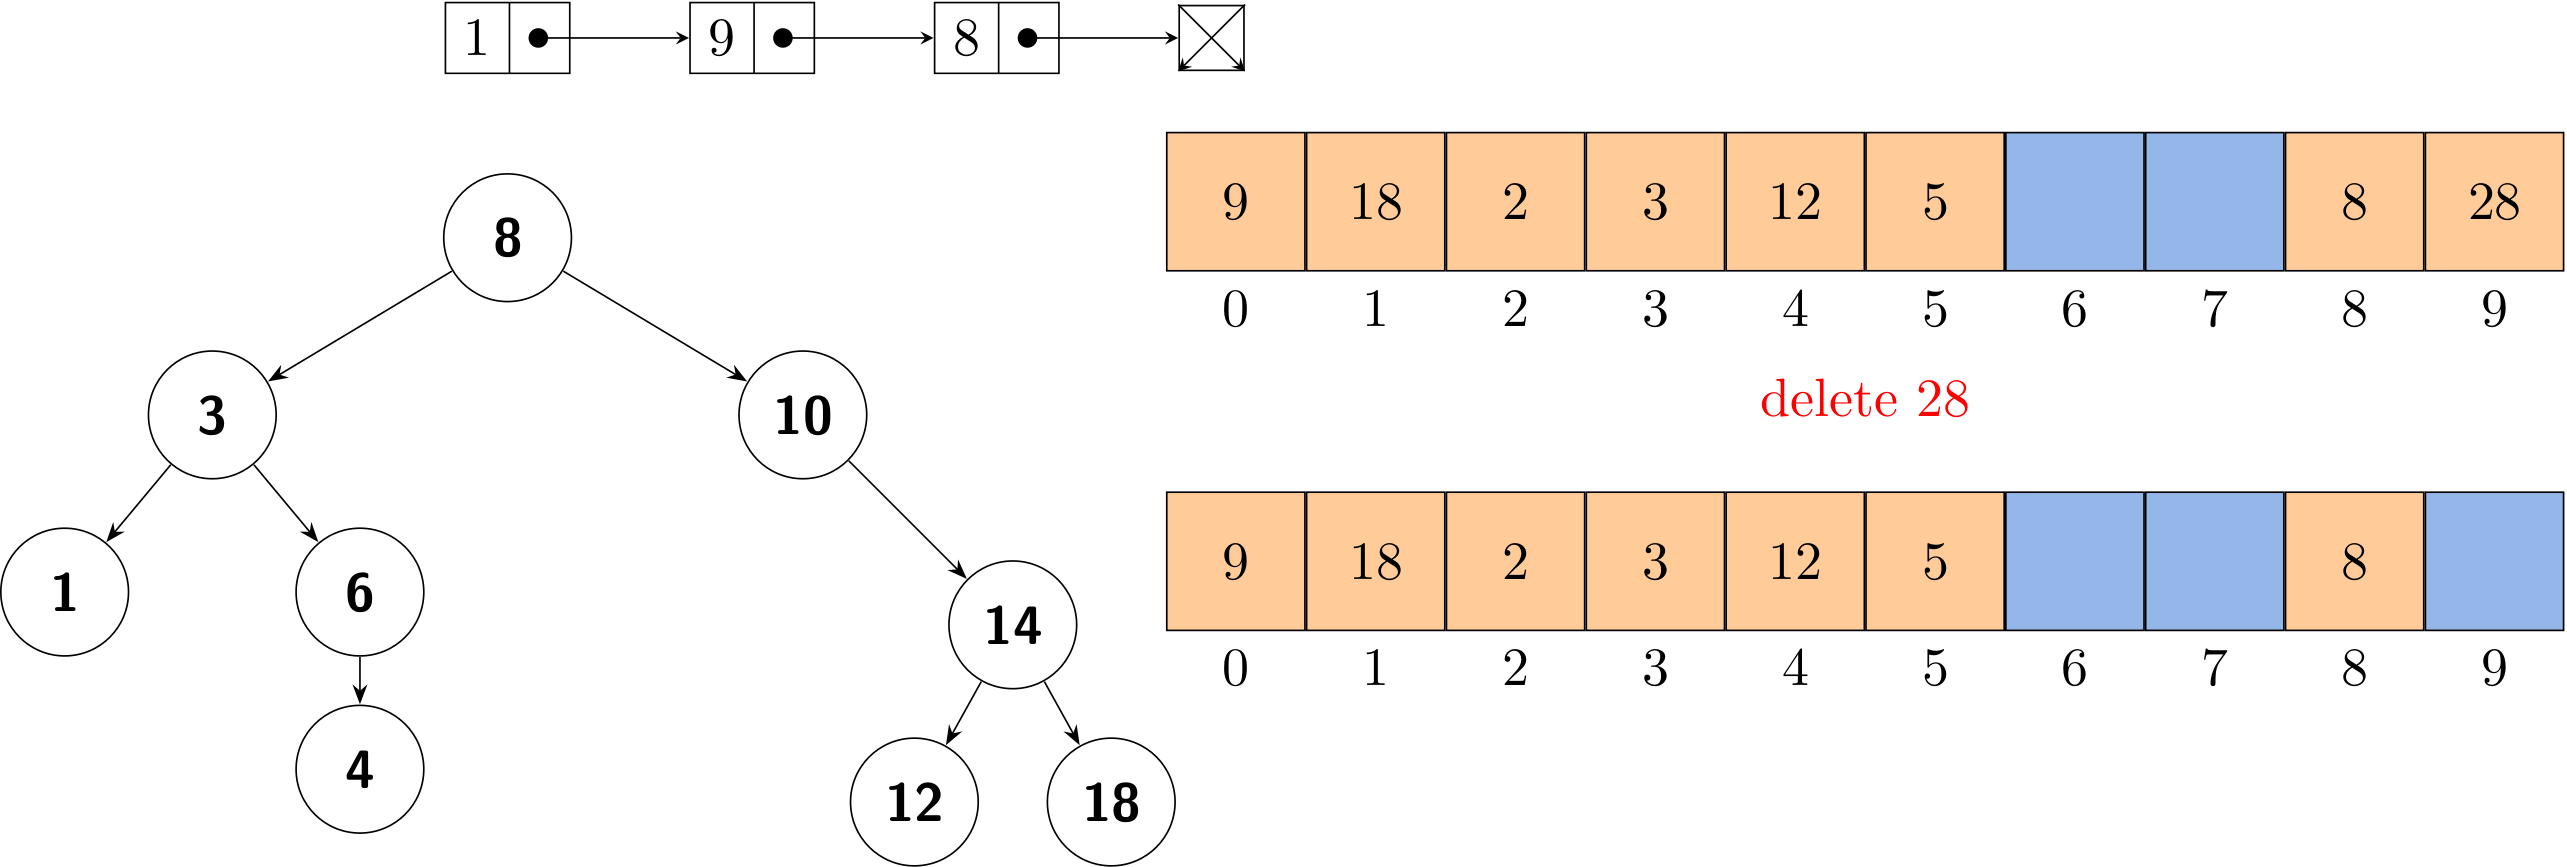
\includegraphics[height=0.7\paperheight]{cover}
% \end{picture}    
% }}
\usebackgroundtemplate{
	\tikz[overlay,remember picture]
	\node[opacity=0.3, at=(current page.south east),anchor=south east, yshift=2cm,xshift=4cm] {
		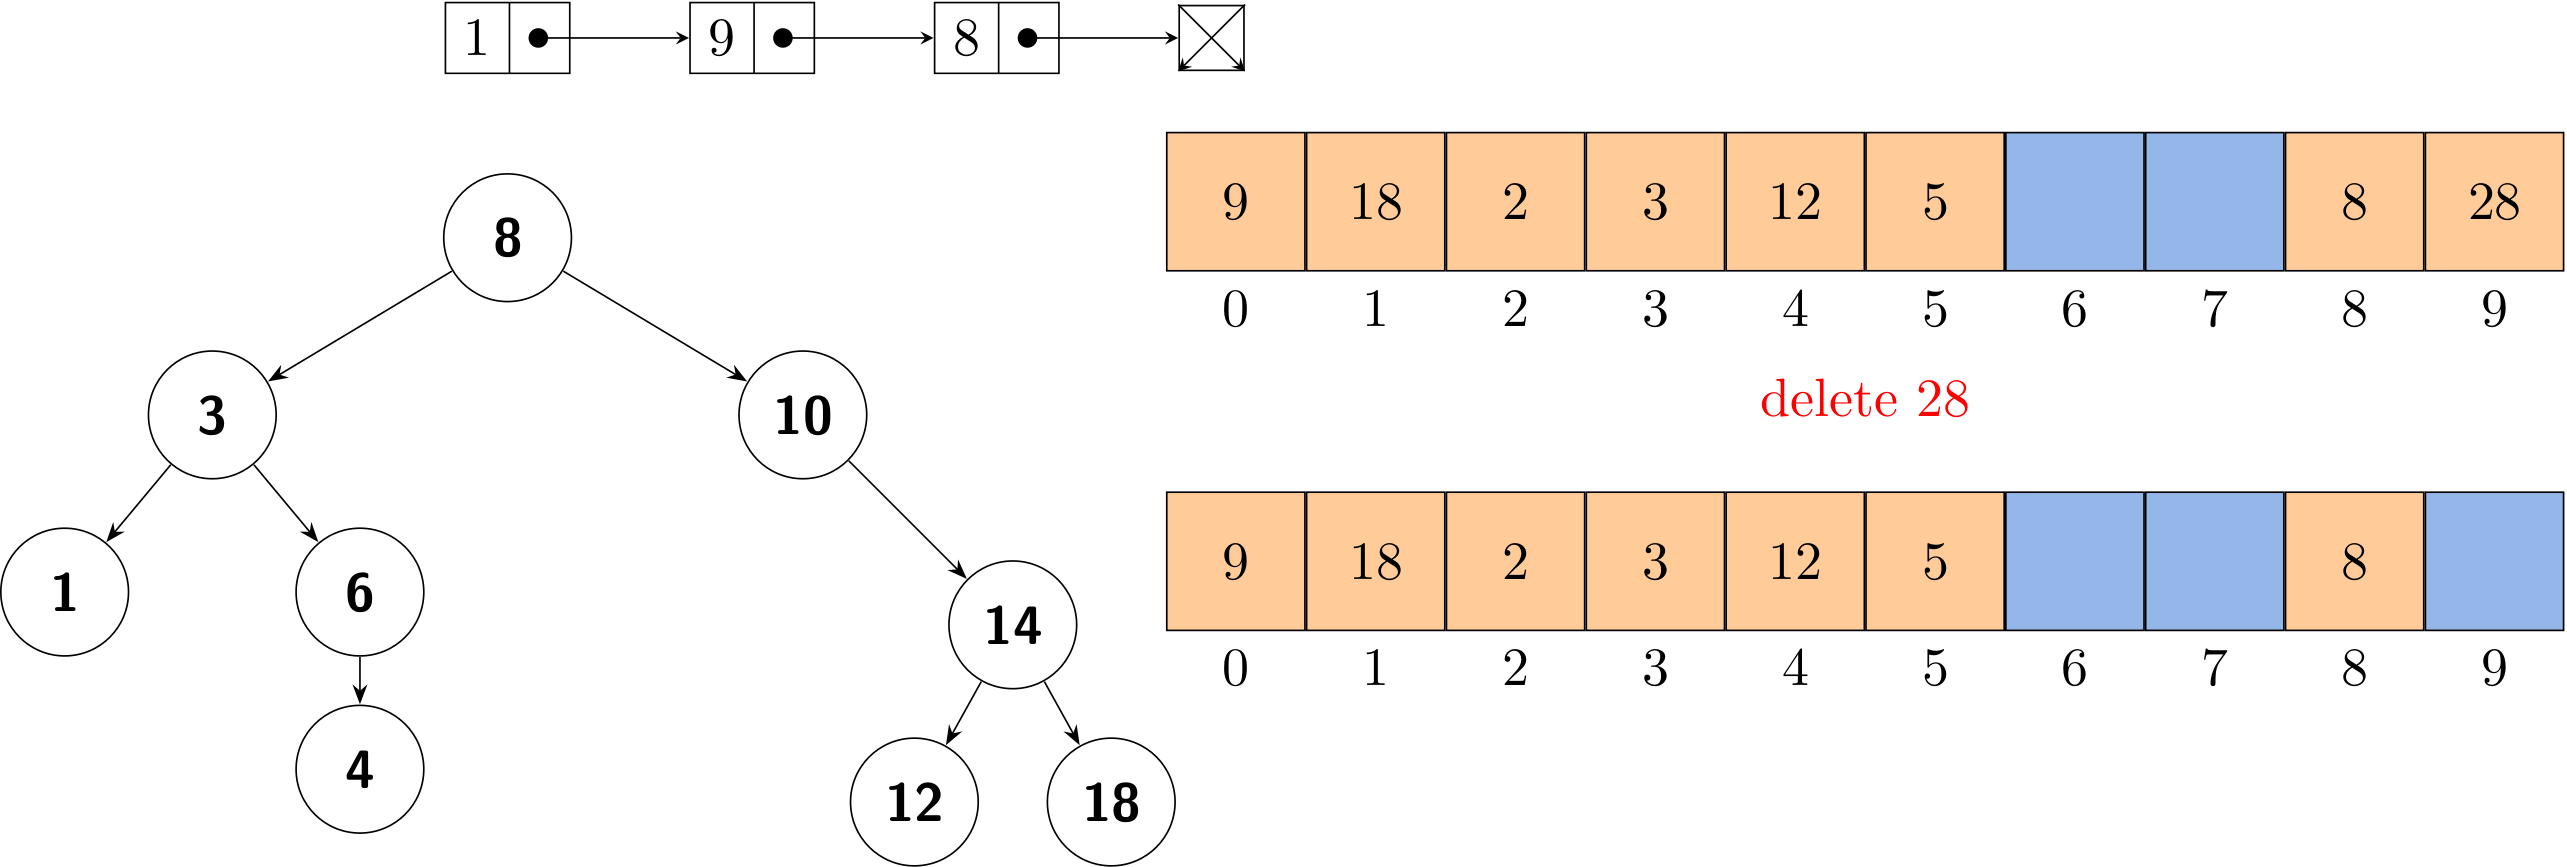
\includegraphics[height=0.6\paperheight]{cover}};
}
\begin{frame}
	\section{\textcolor{darkmidnightblue}{Course Overview}}
\end{frame}

}

%---------------------------------------------------------
%Changing visivility of the text


%---------------------------------------------------------
%Example of the \pause command
\begin{frame}[fragile]
	\frametitle{About Course}
	\begin{exampleblock}{Question}
		\textbf{What are \alert{Data Structures}?}
	\end{exampleblock}

	\begin{displayquote}
		From Cambridge Dictionary: the way in which the parts of a system or object are arranged or organized, or a system arranged in this way
	\end{displayquote}

	\begin{columns}
		\column{0.5\textwidth}
		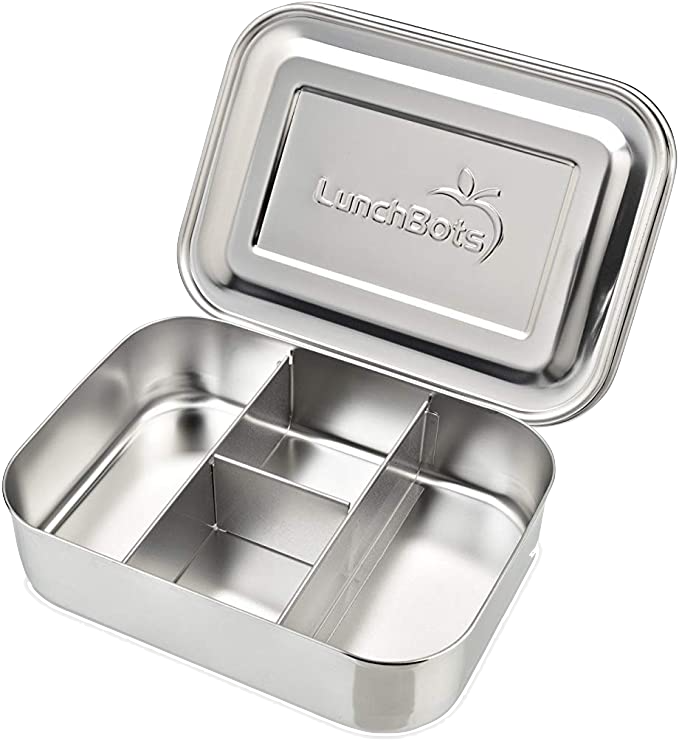
\includegraphics[height=.4\paperheight]{week0/box1}%
		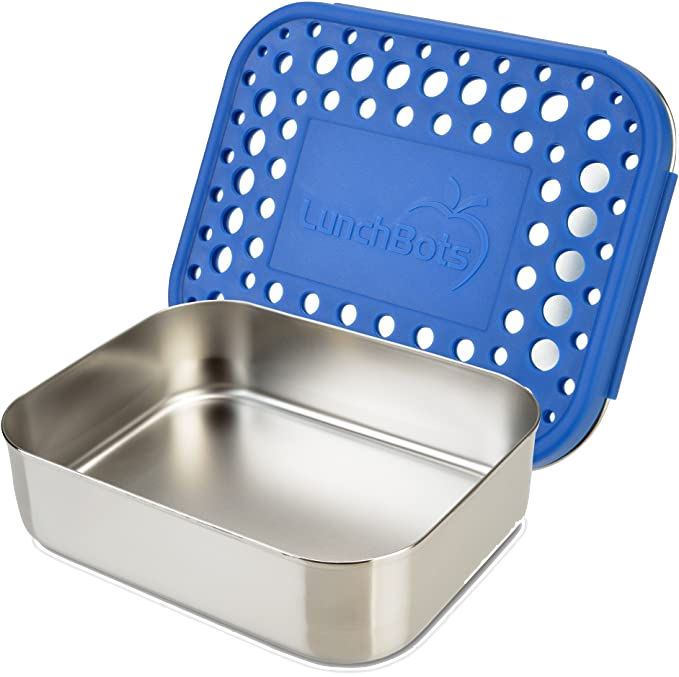
\includegraphics[height=.4\paperheight]{week0/box2}
		\column{.5\textwidth}
		\pause
		In computer science, a data structure is a data \alert{organization, management, and storage} format that is usually chosen for \alert{efficient} access to data.
	\end{columns}

\end{frame}
%---------------------------------------------------------

\begin{frame}[fragile]
	\begin{block}{Fact 1}
		\textbf{Different data structures have varying \alert{capabilities}.}
	\end{block}

	\begin{lstlisting}[language=Java]
List<Book> library = new ArrayList<>();
// add/delete/find book
library.add(new Book("Gone with the wind", 99.0));

String[] books = {"Gone with the Wind", 
                "Hands on Data Structures"};    
\end{lstlisting}

	{\large \faIcon{question-circle}} Can we add a new book onto \emph{books}?
	\pause

	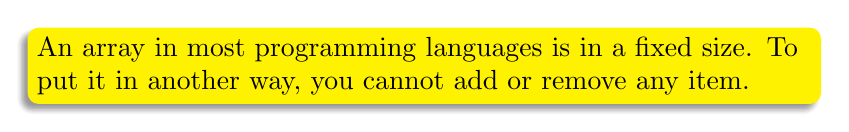
\begin{tikzpicture}
		\node[fill=yellow,blur shadow={shadow xshift=-0.5ex},
			text width=28em,anchor=south west,rounded corners]
		{An array in most programming languages is in a fixed size. To put it in another way, you cannot add or remove any item.};
	\end{tikzpicture}
\end{frame}

\begin{frame}
	\begin{center}
		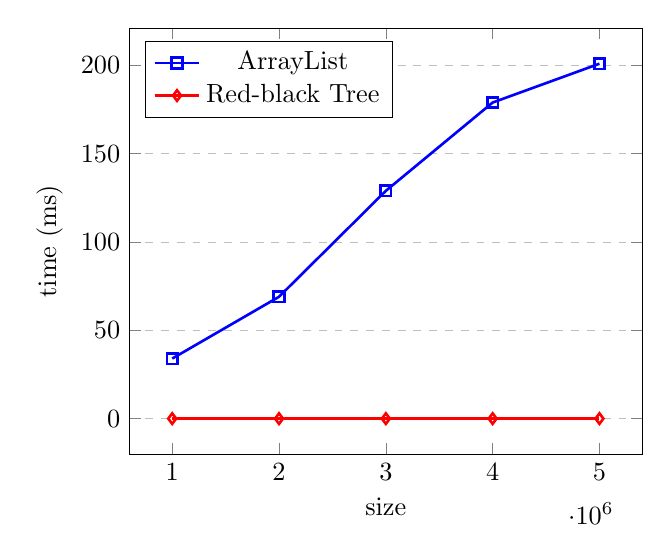
\begin{tikzpicture}[scale=0.95]
			\begin{axis}[
					xlabel={size},
					ylabel={time (ms)},
					ymajorgrids=true,
					grid style=dashed,
					legend pos=north west,
				]
				\addplot[
					color=blue,
					mark=square,
					line width=1pt,
				]
				coordinates {
						(1000000, 34)(2000000, 69)(3000000, 129)(4000000, 179)(5000000, 201)
					};
				\addlegendentry{ArrayList}

				\addplot[color=red,
					mark=diamond,
					line width=1pt,]
				coordinates {
						(1000000, 0)(2000000, 0)(3000000, 0)(4000000, 0)(5000000, 0)
					};
				\addlegendentry{Red-black Tree}

			\end{axis}
		\end{tikzpicture}
	\end{center}
	\begin{block}{Fact 2}
		\textbf{Different data structures have varying \alert{efficiencies}.}
	\end{block}
\end{frame}

\begin{frame}
	\begin{exampleblock}{Question}
		Suppose there are $10^6$ books in an array. To find a book titled \emph{"Gone with the wind"}, how many times is the comparison performed?
		\begin{enumerate}
			\item On the \textbf{best} case;
			\item On the \textbf{worst} case;
			\item On the \textbf{average} case.
		\end{enumerate}
	\end{exampleblock}
\end{frame}

\begin{frame}
	\begin{center}
		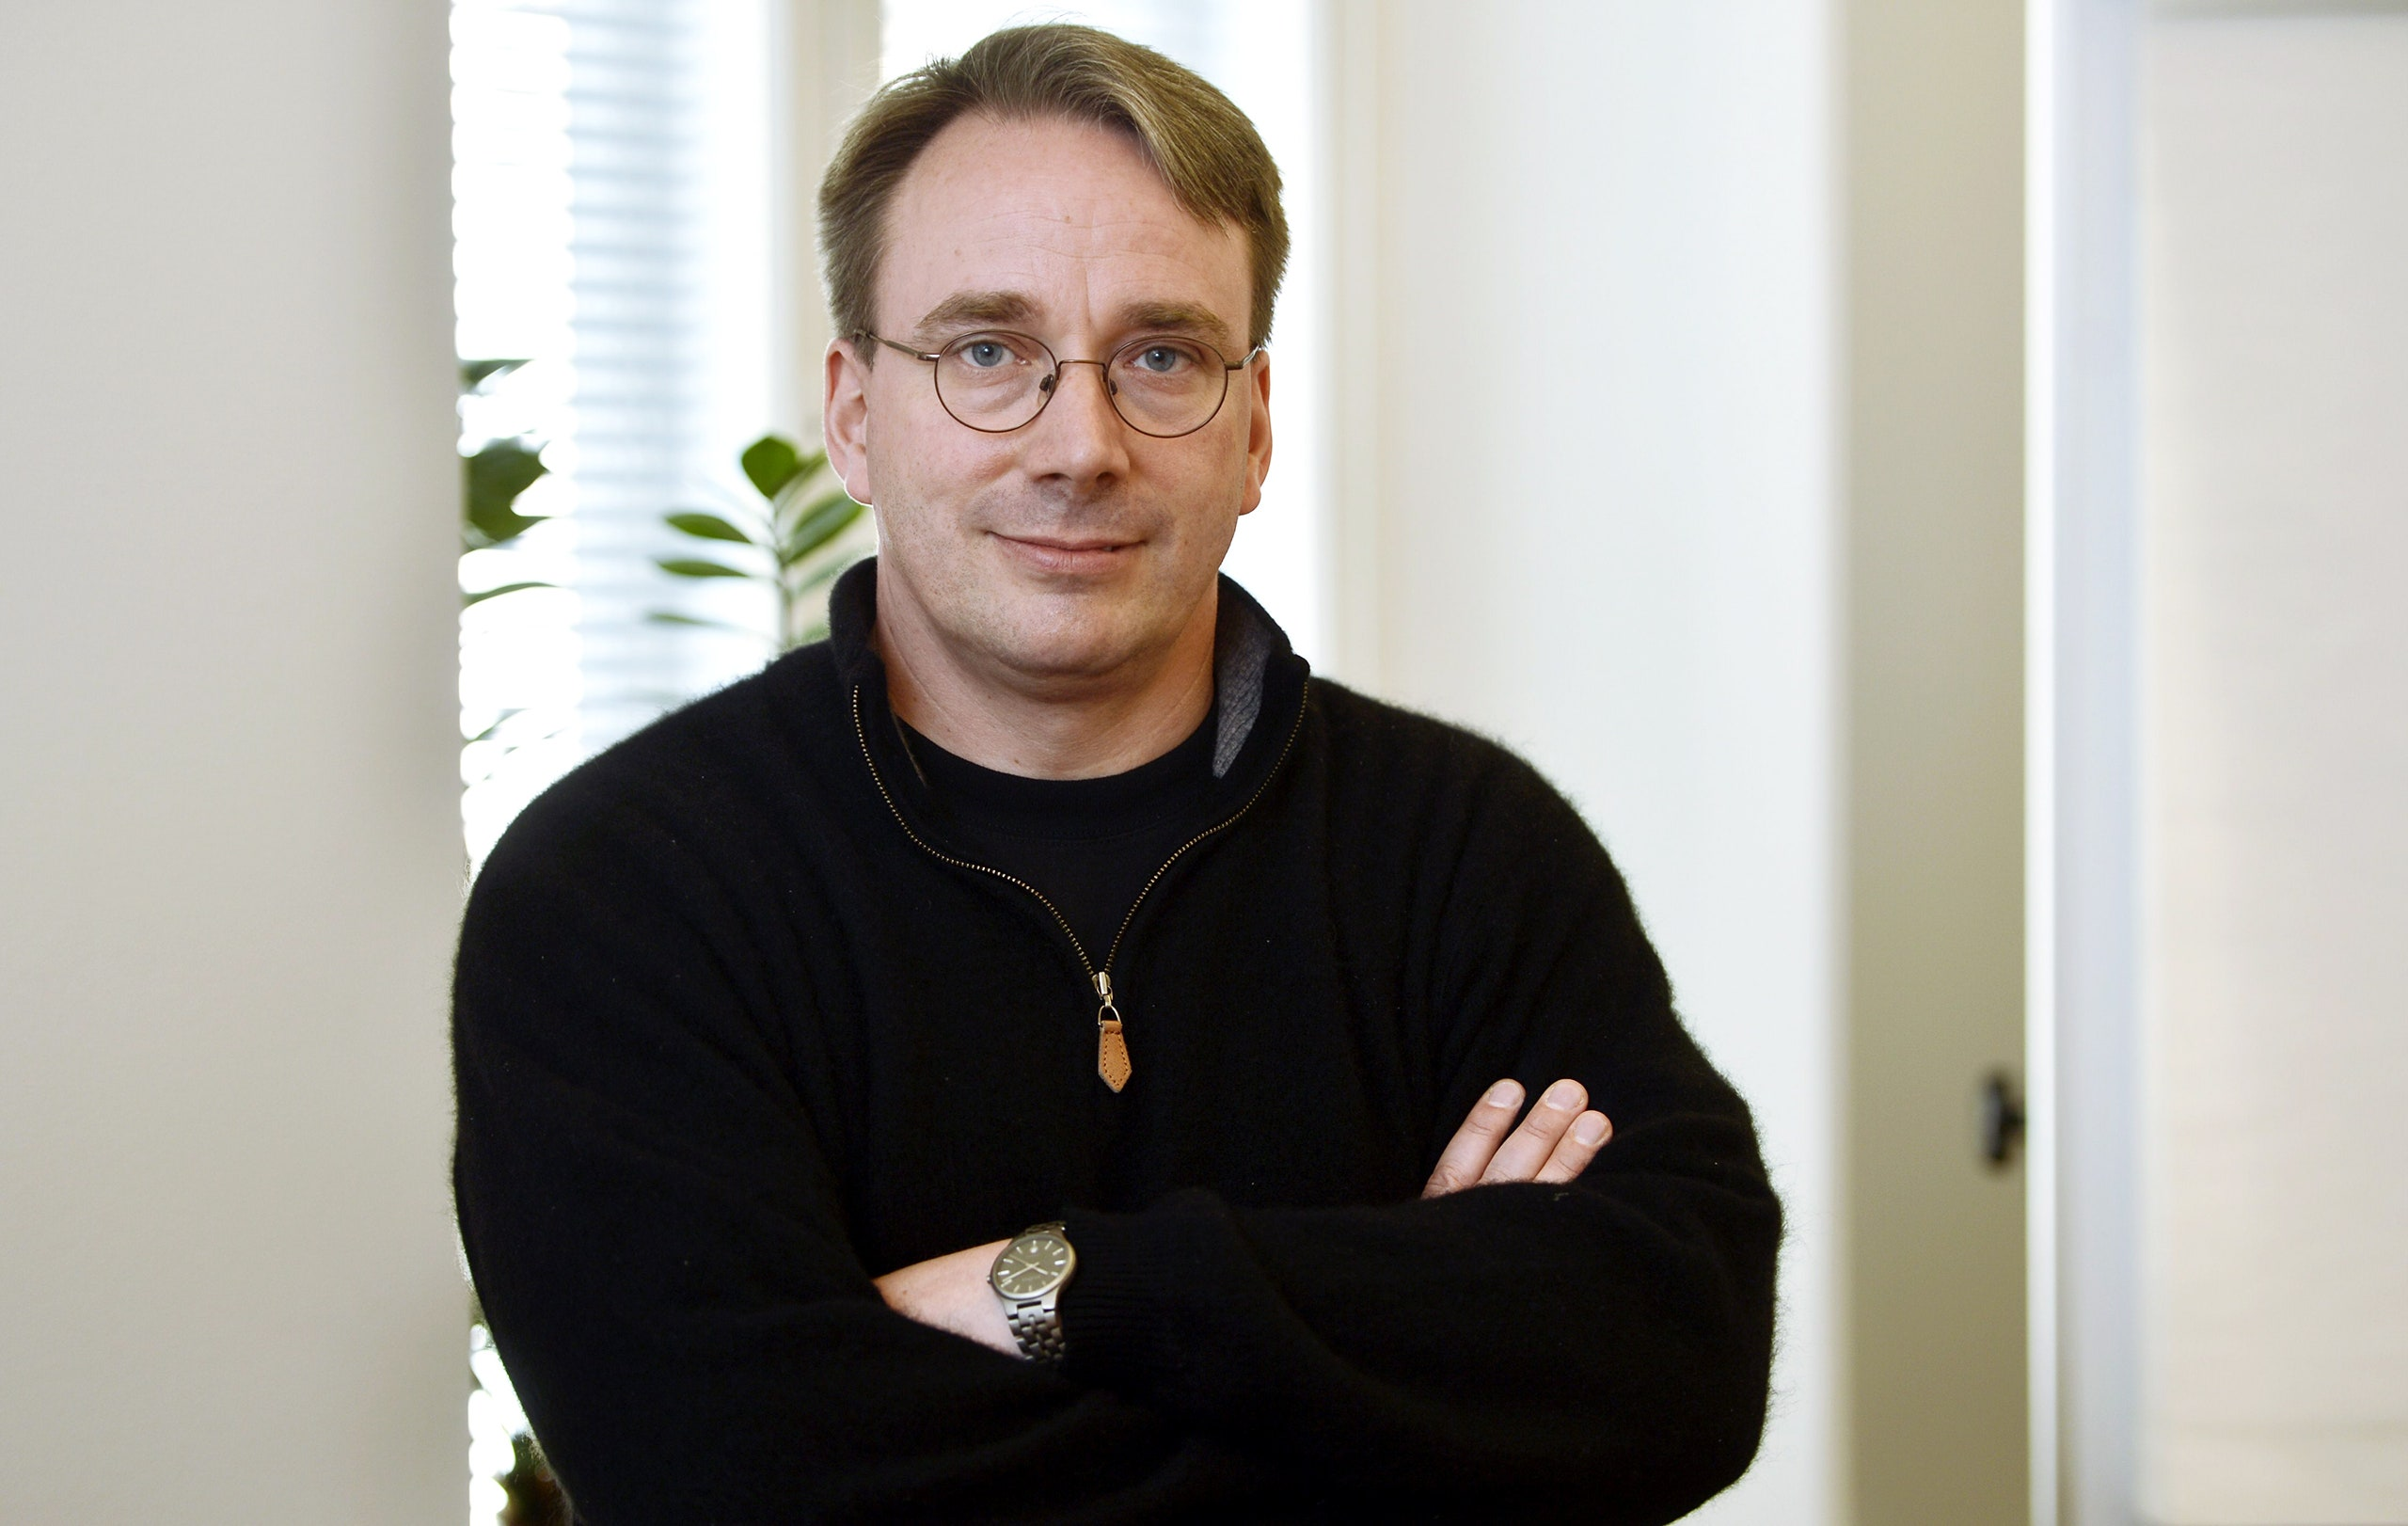
\includegraphics[height=.35\paperheight]{week0/linux}
	\end{center}
	\begin{quote}
		I will, in fact, claim that the difference between a bad programmer and a good one is whether he considers his code or his data structures more important. Bad programmers worry about the code. Good programmers worry about data structures and their relationships.
		\begin{flushright}
			---Linus Torvalds
		\end{flushright}
	\end{quote}
\end{frame}

\begin{frame}{fragile}
	\frametitle{Algorithm}

	$$\mathbf{Data\ Structure + Algorithm = Program}$$

	\begin{quote}
		An algorithm is a finite sequence of rigorous instructions, typically used to solve a class of specific problems or to perform a computation.
	\end{quote}

	Given some \alert{inputs}, an algorithm produces an \alert{output}.

	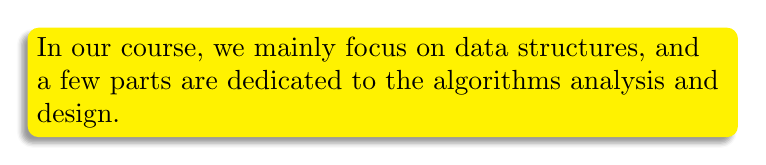
\begin{tikzpicture}
		\node[fill=yellow,blur shadow={shadow xshift=-0.5ex},
			text width=25em,anchor=south west,rounded corners]
		{In our course, we mainly focus on data structures, and a few parts are dedicated to the algorithms analysis and design.};
	\end{tikzpicture}

\end{frame}

\begin{frame}

	\begin{exampleblock}{Example 1}
		Given three positive integers $a$, $b$, $c$, determine whether they can form the sides of a triangle.
	\end{exampleblock}
	If $a + b > c, a + c > b, b + c > a$, then they can form a triangle.
\end{frame}

\begin{frame}
	\begin{exampleblock}{Example 2}
		Given an array of integers, find the maximum element in the array.
	\end{exampleblock}
	\begin{itemize}
		\item Start by initializing the maximum element \alert{max} as the first element in the array.
		\item Iterate through the array, and compare \alert{max} with each element. If the current element is greater than \alert{max}, then replace \alert{max} with the current element.
		\item After the iteration is complete, the final \alert{max} is returned.
	\end{itemize}
\end{frame}

\begin{frame}
	\frametitle{What you will learn}
	\begin{enumerate}
		\item Language built-in data structures
		\item Stack, queue
		\item Linked list
		\item Balanced search tree
		\item Hash table
		\item Graph
	\end{enumerate}
\end{frame}

\begin{frame}
	\frametitle{Prerequisites and tools}
	\begin{outline}
		\1 Skill of a general (\alert{object-oriented}) programming language (e.g., Python, Java).
		\1 High school level of mathematical skills.
		\1 SDK and IDE
		\2 Java: JDK 11 and above; IntelliJ IDEA
		\2 Python: Python 3.7 and above; IntelliJ PyCharm, VSCode, Jupyter Notebook
	\end{outline}
	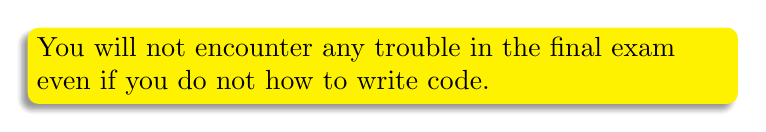
\begin{tikzpicture}
		\node[fill=yellow,blur shadow={shadow xshift=-0.5ex},
			text width=25em,anchor=south west,rounded corners]
		{You will not encounter any trouble in the final exam even if you do not how to write code.};
	\end{tikzpicture}
\end{frame}

\begin{frame}[fragile]
	\frametitle{Pseudo-code}
	Pseudo\textipa{/"sUdoU/}: not genuine; superficially appears to be one thing, but is something else.

	\scalebox{.7}{
		\begin{algorithm}[H]
			\caption{indexOf(a, o)}
			$n\gets a.size()$ \\
			\For{$i\gets 0$ \KwTo $n$}{
				\If{$a[i] == o$}{
					\Return{i}
				}
			}
			\Return{-1}
		\end{algorithm}
	}
\end{frame}

\begin{frame}
	\frametitle{Books}
	\begin{enumerate}
		\item \alert{Introduction to Algorithms} by Thomas H. Cormen, Charles E. Leiserson, Ronald L. Rivest, and Clifford Stein.
		\item \alert{Algorithms} by Robert Sedgewick, Kevin Wayne.
		\item \alert{Data Structures and Algorithms in Java} by Michael T. Goodrich, Roberto Tamassia, Michael H. Goldwasser.
		\item \alert{Data Structures and Algorithms in Python} by Michael T. Goodrich, Roberto Tamassia, Michael H. Goldwasser.
	\end{enumerate}
	\textbf{\href{https://chenzhongpu.github.io/data-structure-swufe/}{Hands On Data Structures}} by me.
\end{frame}

\begin{frame}
	\frametitle{Resources}
	\begin{itemize}
		\item Slides and code (\url{https://github.com/ChenZhongPu/data-structure-swufe})
		\item TA: HAO Wanjun(郝万钧)
		\item Google, ChatGPT, Claude (\url{https://claude.ai}), Poe (\url{https://poe.com})
	\end{itemize}
	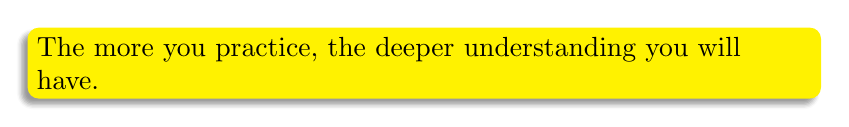
\begin{tikzpicture}
		\node[fill=yellow,blur shadow={shadow xshift=-0.5ex},
			text width=28em,anchor=south west,rounded corners]
		{The more you practice, the deeper understanding you will have.};
	\end{tikzpicture}
\end{frame}

\begin{frame}[fragile]
	\frametitle{Evaluation}

	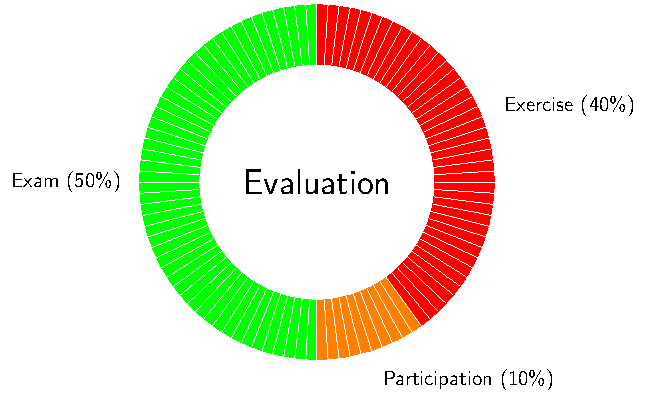
\includegraphics[height=.6\paperheight]{week0/evaluation}

	
\begin{tikzpicture}
		\node[fill=red!80, text=white, blur shadow={shadow xshift=-0.5ex},
			text width=15em,anchor=south west,rounded corners, ]
		{Plagiarism is strictly prohibited!
		};
	\end{tikzpicture}
\end{frame}

\end{document}
